\section{\texttt{clickhouse-backup} performance test}
\label{app:chbk-perf}
While backing up and uploading a backup to remote storage
seemed to work fine (see \ref{app:ch-perf}),
we were unable to actually recover from the backup.
Several attempts were made at restoring from or downloading the remote backups.
All were unsuccessful.
Errors occured during the download phase of the recovery.

An attempt was made to back up up a single table,
upload it to remote storage and then restore from it.
This attempt was successful, but only used a tiny amount of data.
This, and the fact that we were able to list remote backups,
indicates that the configuration/connection to the remote storage itself was probably fine.

Unfortunately, we were not able to perform a proper
performance test of \texttt{clickhouse-backup} with 1TB of data.

\subsection{Recovery with \texttt{clickhouse-backup} (first set of attempts)}
\label{sec:org4d2ee6b}
\subsubsection{Rebuild VM}
\label{sec:org0452162}
Delete VM:
\begin{minted}[breaklines=true,breakanywhere=true]{powershell}
# Delete the VM
az vm delete --name $CHName --resource-group $RGName --yes

# Get all resources in resource group
$resources = az resource list --resource-group $RGName | ConvertFrom-Json -AsHashtable

# Fetch only the ids of resources with names containing "Clickhouse".
$filtered = foreach($r in $resources) {
    Write-Output $r["id"] | grep Clickhouse
}

# Delete the resources
$filtered | % {Remove-AzResource -ResourceId $_ -Force}
$filtered | % {Remove-AzResource -ResourceId $_ -Force}
\end{minted}

Create VM:
\begin{minted}[breaklines=true,breakanywhere=true]{powershell}
az vm create `
    --resource-group $RGName `
    --name $CHName `
    --image Canonical:UbuntuServer:16.04-LTS:16.04.202109280 `
    --admin-username azureuser `
    --size Standard_D4s_v4 `
    --os-disk-size-gb 2048 `
    --ssh-key-values $SSHPath `
    --public-ip-sku Standard
\end{minted}

Install ClickHouse:
\begin{minted}[breaklines=true,breakanywhere=true]{bash}
sudo apt-get install -y apt-transport-https ca-certificates dirmngr
sudo apt-key adv --keyserver hkp://keyserver.ubuntu.com:80 --recv 8919F6BD2B48D754

echo "deb https://packages.clickhouse.com/deb stable main" | sudo tee \
    /etc/apt/sources.list.d/clickhouse.list
sudo apt-get update

sudo apt-get install -y clickhouse-server clickhouse-client

sudo clickhouse start
sudo service clickhouse-server start
\end{minted}

Install \texttt{clickhouse-backup}:
\begin{minted}[breaklines=true,breakanywhere=true]{bash}
# Download archive containing binary
wget https://github.com/AlexAkulov/clickhouse-backup/releases/download/v1.3.2/clickhouse-backup-linux-amd64.tar.gz

# Decompress archive
tar -zxvf clickhouse-backup-linux-amd64.tar.gz

# Move binary to home directory
mv build/linux/amd64/clickhouse-backup ~

# Cleanup
rmdir -p build/linux/amd64
rm clickhouse-backup-linux-amd64.tar.gz
\end{minted}

\texttt{config.yaml} was copied from the test environment (see \ref{app:ch-perf}).

\texttt{config.yaml}:
\begin{minted}[breaklines=true,breakanywhere=true]{yaml}
general:
  remote_storage: azblob
  max_file_size: 0
  disable_progress_bar: false
  backups_to_keep_local: 0
  backups_to_keep_remote: 0
  log_level: info
  allow_empty_backups: false
  download_concurrency: 1
  upload_concurrency: 1
  restore_schema_on_cluster: ""
  upload_by_part: true
  download_by_part: true
clickhouse:
  username: default
  password: ""
  host: localhost
  port: 9000
  disk_mapping: {}
  skip_tables:
  - system.*
  - INFORMATION_SCHEMA.*
  - information_schema.*
  timeout: 5m
  freeze_by_part: false
  secure: false
  skip_verify: false
  sync_replicated_tables: false
  log_sql_queries: true
  config_dir: /etc/clickhouse-server/
  restart_command: systemctl restart clickhouse-server
  ignore_not_exists_error_during_freeze: true
  tls_key: ""
  tls_cert: ""
  tls_ca: ""
  debug: false
s3:
  access_key: ""
  secret_key: ""
  bucket: ""
  endpoint: ""
  region: us-east-1
  acl: private
  assume_role_arn: ""
  force_path_style: false
  path: ""
  disable_ssl: false
  compression_level: 1
  compression_format: tar
  sse: ""
  disable_cert_verification: false
  storage_class: STANDARD
  concurrency: 1
  part_size: 0
  max_parts_count: 10000
  debug: false
gcs:
  credentials_file: ""
  credentials_json: ""
  bucket: ""
  path: ""
  compression_level: 1
  compression_format: tar
  debug: false
  endpoint: ""
cos:
  url: ""
  timeout: 2m
  secret_id: ""
  secret_key: ""
  path: ""
  compression_format: tar
  compression_level: 1
  debug: false
api:
  listen: localhost:7171
  enable_metrics: true
  enable_pprof: false
  username: ""
  password: ""
  secure: false
  certificate_file: ""
  private_key_file: ""
  create_integration_tables: false
  allow_parallel: false
ftp:
  address: ""
  timeout: 2m
  username: ""
  password: ""
  tls: false
  path: ""
  compression_format: tar
  compression_level: 1
  concurrency: 1
  debug: false
sftp:
  address: ""
  port: 22
  username: ""
  password: ""
  key: ""
  path: ""
  compression_format: tar
  compression_level: 1
  concurrency: 1
  debug: false
azblob:
  endpoint_suffix: core.windows.net
  account_name: "perfchbksa"
  account_key: "EIhee0y3zertAVbAa7cRAhYQ/2Oui25vdr6DoL05qkA+CfZZpFMlabzJFPtJG8Xdc735PAbA8w8r+AStl89ieA=="
  sas: "se=2022-05-18&sp=racwdl&sv=2021-04-10&sr=c&skoid=d404139d-e156-421c-9450-19e9734a8141&sktid=09a10672-822f-4467-a5ba-5bb375967c05&skt=2022-05-11T07%3A01%3A18Z&ske=2022-05-18T00%3A00%3A00Z&sks=b&skv=2021-04-10&sig=GgFsZifUWr0r71gCZaD9PbxRXrybhWS09Hpb2scfsKg%3D"
  use_managed_identity: false
  container: "chbkperfcontainer"
  path: "https://perfchbksa.blob.core.windows.net/chbkperfcontainer"
  compression_level: 1
  compression_format: tar
  sse_key: ""
  buffer_size: 0
  buffer_count: 3
  max_parts_count: 1
\end{minted}
\subsubsection{Try to restore from remote backup}
\label{sec:org5cb0fa6}
Bash commands were performed as root in \path{/home/azureuser}.
SQL statements were performed in \texttt{clickhouse-client}.

Showing the tables in the database (no tables):
\begin{minted}[breaklines=true,breakanywhere=true]{sql}
SHOW TABLES

-- Query id: e41781d1-477e-4d48-be0c-73e3b5f26eaa
--
-- Ok.
--
-- 0 rows in set. Elapsed: 0.002 sec.
\end{minted}

Listing remote backups:
\begin{minted}[breaklines=true,breakanywhere=true]{bash}
./clickhouse-backup list remote --config ./config.yaml
# 2022/05/12 09:39:48.379024  info SELECT max(toInt64(bytes_on_disk * 1.02)) AS max_file_size FROM system.parts
# 2022-05-11T07-25-16   895.29GiB   11/05/2022 10:44:05   remote      tar
\end{minted}

Restoring from the remote backup:
\begin{minted}[breaklines=true,breakanywhere=true]{bash}
time ./clickhouse-backup restore_remote 2022-05-11T07-25-16 --config ./config.yaml

# 2022/05/12 09:48:21.324699  info SELECT value FROM `system`.`build_options` where name='VERSION_INTEGER'
# 2022/05/12 09:48:21.326557  info SELECT * FROM system.disks;
# 2022/05/12 09:48:21.332100  info SELECT max(toInt64(bytes_on_disk * 1.02)) AS max_file_size FROM system.parts
# 2022/05/12 09:48:21.459701  info done                      backup=2022-05-11T07-25-16 duration=54ms operation=download size=3.36KiB table_metadata=default.github_events1
# 2022/05/12 09:48:21.507383  info done                      backup=2022-05-11T07-25-16 duration=48ms operation=download size=3.32KiB table_metadata=default.github_events2
# 2022/05/12 09:48:21.512022  info done                      backup=2022-05-11T07-25-16 duration=5ms operation=download size=3.36KiB table_metadata=default.github_events3
# 2022/05/12 09:48:21.516128  info done                      backup=2022-05-11T07-25-16 duration=4ms operation=download size=3.32KiB table_metadata=default.github_events4
# 2022/05/12 09:48:21.520984  info done                      backup=2022-05-11T07-25-16 duration=5ms operation=download size=3.28KiB table_metadata=default.github_events5
# 2022/05/12 09:49:21.524887 error can't acquire semaphore during downloadTableData: context canceled---------]  57.67% 59s
# 2022/05/12 09:49:21.642779 error can't acquire semaphore during Download: context canceled backup=2022-05-11T07-25-16 operation=download
# 2022/05/12 09:50:21.672318 error can't acquire semaphore during downloadTableData: context canceled---------]   8.04% 59s
# 2022/05/12 09:50:21.770237 error one of Download go-routine return error: one of downloadTableData go-routine return error: handling file: /all_3441_4218_4/file_time.bin: context deadline exceeded
#
# real    2m0.461s
# user    0m10.068s
# sys     0m14.108s
\end{minted}

The restoration failed.
\subsubsection{Try to download remote backup}
\label{sec:org8b2d881}
Since \texttt{clickhouse-backup restore\_remote} failed,
we tried to instead download the backup first, and then restore afterwards.
This also failed with the same error.

\begin{minted}[breaklines=true,breakanywhere=true]{bash}
time ./clickhouse-backup download 2022-05-11T07-25-16 --config ./config.yaml

# 2022/05/12 10:00:42.788222  info SELECT value FROM `system`.`build_options` where name='VERSION_INTEGER'
# 2022/05/12 10:00:42.790756  info SELECT * FROM system.disks;
# 2022/05/12 10:00:42.797256  info SELECT max(toInt64(bytes_on_disk * 1.02)) AS max_file_size FROM system.parts
# 2022/05/12 10:00:42.846572  info done                      backup=2022-05-11T07-25-16 duration=5ms operation=download size=3.36KiB table_metadata=default.github_events1
# 2022/05/12 10:00:42.853218  info done                      backup=2022-05-11T07-25-16 duration=7ms operation=download size=3.32KiB table_metadata=default.github_events2
# 2022/05/12 10:00:42.857772  info done                      backup=2022-05-11T07-25-16 duration=4ms operation=download size=3.36KiB table_metadata=default.github_events3
# 2022/05/12 10:00:42.864379  info done                      backup=2022-05-11T07-25-16 duration=7ms operation=download size=3.32KiB table_metadata=default.github_events4
# 2022/05/12 10:00:42.869284  info done                      backup=2022-05-11T07-25-16 duration=5ms operation=download size=3.28KiB table_metadata=default.github_events5
# 2022/05/12 10:01:42.873871 error can't acquire semaphore during downloadTableData: context canceled---------]  63.84% 59s
# 2022/05/12 10:01:42.966195 error can't acquire semaphore during Download: context canceled backup=2022-05-11T07-25-16 operation=download
# 2022/05/12 10:02:43.002110 error can't acquire semaphore during downloadTableData: context canceled---------]   8.08% 59s
# 2022/05/12 10:02:43.087969 error one of Download go-routine return error: one of downloadTableData go-routine return error: handling file: /all_3441_4218_4/file_time.bin: context deadline exceeded
#
# real    2m0.314s
# user    0m10.550s
# sys     0m12.509s
\end{minted}
\subsubsection{Rebuild VM again}
\label{sec:org56a63e8}
The VM was once again rebuilt,
in the same way as in \hyperref[sec:org0452162]{Rebuild VM}.
\subsubsection{Download remote backup again (third attempt)}
\label{sec:org3f5a3c3}
Tried to download the remote backup again, like in \hyperref[sec:org8b2d881]{Try to download remote backup},
but it failed once again.
\subsection{Recovery with \texttt{clickhouse-backup} (second set of attempts)}
\label{sec:orgfaf1fce}
We had another go at restoring from the remote \texttt{clickhouse-backup} backups.
Downloading/restoring from remote backups
failed once again, and we were not sure what to do about it.

We made an attempt at uploading a very small backup to remote storage and then recovering from it.
This worked fine.

Finally, we made an attempt at recovering from the local version of the remote backup.
This worked well.
The restoration took only 2.687 seconds.

\subsubsection{Restore VM}
\label{sec:org46296f4}
The VM was restored via Azure Backup.
This process is the same as in [cref].
\subsubsection{Drop tables}
\label{sec:org5bece9d}
Make it possible to drop tables (had to be run between drop table statements):
\begin{minted}[breaklines=true,breakanywhere=true]{bash}
sudo touch '/var/lib/clickhouse/flags/force_drop_table' && sudo chmod 666 '/var/lib/clickhouse/flags/force_drop_table'
\end{minted}

\begin{minted}[breaklines=true,breakanywhere=true]{sql}
DROP TABLE github_events1
DROP TABLE github_events2
DROP TABLE github_events3
DROP TABLE github_events4
DROP TABLE github_events5
\end{minted}
\subsubsection{Download backup}
\label{sec:org25a0557}
Commands were performed as root.

List remote backups:
\begin{minted}[breaklines=true,breakanywhere=true]{bash}
./clickhouse-backup list remote --config config.yaml
# 2022/05/14 10:00:29.509778  info SELECT max(toInt64(bytes_on_disk * 1.02)) AS max_file_size FROM system.parts
# 2022-05-11T07-25-16   895.29GiB   11/05/2022 10:44:05   remote      tar
\end{minted}

Drop
\begin{minted}[breaklines=true,breakanywhere=true]{bash}
./clickhouse-backup delete local 2022-05-11T07-25-16
\end{minted}

Restore from remote backup:
\begin{minted}[breaklines=true,breakanywhere=true]{bash}
time ./clickhouse-backup restore_remote 2022-05-11T07-25-16 --config config.yaml
# 2022/05/14 10:04:26.068449  info SELECT value FROM `system`.`build_options` where name='VERSION_INTEGER'
# 2022/05/14 10:04:26.071514  info SELECT * FROM system.disks;
# 2022/05/14 10:04:26.078712  info SELECT max(toInt64(bytes_on_disk * 1.02)) AS max_file_size FROM system.parts
# 2022/05/14 10:04:26.202816  info done                      backup=2022-05-11T07-25-16 duration=54ms operation=download size=3.36KiB table_metadata=default.github_events1
# 2022/05/14 10:04:26.207742  info done                      backup=2022-05-11T07-25-16 duration=5ms operation=download size=3.32KiB table_metadata=default.github_events2
# 2022/05/14 10:04:26.220053  info done                      backup=2022-05-11T07-25-16 duration=12ms operation=download size=3.36KiB table_metadata=default.github_events3
# 2022/05/14 10:04:26.225487  info done                      backup=2022-05-11T07-25-16 duration=5ms operation=download size=3.32KiB table_metadata=default.github_events4
# 2022/05/14 10:04:26.230170  info done                      backup=2022-05-11T07-25-16 duration=5ms operation=download size=3.28KiB table_metadata=default.github_events5
# 2022/05/14 10:05:26.234385 error can't acquire semaphore during downloadTableData: context canceled---------]  66.83% 59s
# 2022/05/14 10:05:26.314936 error can't acquire semaphore during Download: context canceled backup=2022-05-11T07-25-16 operation=download
# 2022/05/14 10:06:26.354581 error can't acquire semaphore during downloadTableData: context canceled---------]   9.17% 59s
# 2022/05/14 10:06:26.452971 error one of Download go-routine return error: one of downloadTableData go-routine return error: handling file: /all_3441_4218_4/merge_commit_sha.bin: context deadline exceeded
#
# real    2m0.400s
# user    0m11.283s
# sys     0m14.051s
\end{minted}
\subsubsection{Test with a smaller amount of data (not measuring performance)}
\label{sec:orgbd12c9f}
We did a test where we backup up and recovered a small amount of data,
to prove that the configuration was valid.

Create empty table:
\begin{minted}[breaklines=true,breakanywhere=true]{sql}
CREATE TABLE github_events1
(
    file_time DateTime,
    event_type Enum('CommitCommentEvent' = 1, 'CreateEvent' = 2, 'DeleteEvent' = 3, 'ForkEvent' = 4,
                    'GollumEvent' = 5, 'IssueCommentEvent' = 6, 'IssuesEvent' = 7, 'MemberEvent' = 8,
                    'PublicEvent' = 9, 'PullRequestEvent' = 10, 'PullRequestReviewCommentEvent' = 11,
                    'PushEvent' = 12, 'ReleaseEvent' = 13, 'SponsorshipEvent' = 14, 'WatchEvent' = 15,
                    'GistEvent' = 16, 'FollowEvent' = 17, 'DownloadEvent' = 18, 'PullRequestReviewEvent' = 19,
                    'ForkApplyEvent' = 20, 'Event' = 21, 'TeamAddEvent' = 22),
    actor_login LowCardinality(String),
    repo_name LowCardinality(String),
    created_at DateTime,
    updated_at DateTime,
    action Enum('none' = 0, 'created' = 1, 'added' = 2, 'edited' = 3, 'deleted' = 4, 'opened' = 5, 'closed' = 6, 'reopened' = 7, 'assigned' = 8, 'unassigned' = 9,
                'labeled' = 10, 'unlabeled' = 11, 'review_requested' = 12, 'review_request_removed' = 13, 'synchronize' = 14, 'started' = 15, 'published' = 16, 'update' = 17, 'create' = 18, 'fork' = 19, 'merged' = 20),
    comment_id UInt64,
    body String,
    path String,
    position Int32,
    line Int32,
    ref LowCardinality(String),
    ref_type Enum('none' = 0, 'branch' = 1, 'tag' = 2, 'repository' = 3, 'unknown' = 4),
    creator_user_login LowCardinality(String),
    number UInt32,
    title String,
    labels Array(LowCardinality(String)),
    state Enum('none' = 0, 'open' = 1, 'closed' = 2),
    locked UInt8,
    assignee LowCardinality(String),
    assignees Array(LowCardinality(String)),
    comments UInt32,
    author_association Enum('NONE' = 0, 'CONTRIBUTOR' = 1, 'OWNER' = 2, 'COLLABORATOR' = 3, 'MEMBER' = 4, 'MANNEQUIN' = 5),
    closed_at DateTime,
    merged_at DateTime,
    merge_commit_sha String,
    requested_reviewers Array(LowCardinality(String)),
    requested_teams Array(LowCardinality(String)),
    head_ref LowCardinality(String),
    head_sha String,
    base_ref LowCardinality(String),
    base_sha String,
    merged UInt8,
    mergeable UInt8,
    rebaseable UInt8,
    mergeable_state Enum('unknown' = 0, 'dirty' = 1, 'clean' = 2, 'unstable' = 3, 'draft' = 4),
    merged_by LowCardinality(String),
    review_comments UInt32,
    maintainer_can_modify UInt8,
    commits UInt32,
    additions UInt32,
    deletions UInt32,
    changed_files UInt32,
    diff_hunk String,
    original_position UInt32,
    commit_id String,
    original_commit_id String,
    push_size UInt32,
    push_distinct_size UInt32,
    member_login LowCardinality(String),
    release_tag_name String,
    release_name String,
    review_state Enum('none' = 0, 'approved' = 1, 'changes_requested' = 2, 'commented' = 3, 'dismissed' = 4, 'pending' = 5)
)
ENGINE = MergeTree
ORDER BY (event_type, repo_name, created_at)
\end{minted}

Create local backup:
\begin{minted}[breaklines=true,breakanywhere=true]{bash}
./clickhouse-backup create
# 2022/05/14 10:12:59.474330  info SELECT name, engine FROM system.databases WHERE name NOT IN ('system', 'INFORMATION_SCHE
# MA', 'information_schema')
# 2022/05/14 10:12:59.477846  info SHOW CREATE DATABASE `default`
# 2022/05/14 10:12:59.481048  info SELECT count() FROM system.settings WHERE name = 'show_table_uuid_in_table_create_query_
# if_not_nil'
# 2022/05/14 10:12:59.483473  info SELECT name FROM system.databases WHERE engine IN ('MySQL','PostgreSQL')
# 2022/05/14 10:12:59.485660  info
#                 SELECT
#                         countIf(name='data_path') is_data_path_present,
#                         countIf(name='data_paths') is_data_paths_present,
#                         countIf(name='uuid') is_uuid_present,
#                         countIf(name='create_table_query') is_create_table_query_present,
#                         countIf(name='total_bytes') is_total_bytes_present
#                 FROM system.columns WHERE database='system' AND table='tables'
#
# 2022/05/14 10:12:59.488383  info SELECT database, name, engine , data_paths , uuid , create_table_query , coalesce(total_
# bytes, 0) AS total_bytes   FROM system.tables WHERE is_temporary = 0 SETTINGS show_table_uuid_in_table_create_query_if_no
# t_nil=1
# 2022/05/14 10:12:59.496461  info SELECT sum(bytes_on_disk) as size FROM system.parts WHERE database='default' AND table='
# github_events1' GROUP BY database, table
# 2022/05/14 10:12:59.502336  info SELECT value FROM `system`.`build_options` where name='VERSION_INTEGER'
# 2022/05/14 10:12:59.505121  info SELECT * FROM system.disks;
# 2022/05/14 10:12:59.508045  info ALTER TABLE `default`.`github_events1` FREEZE WITH NAME 'b380781a01ec426e8493f83f940e7f5
# 8';
# 2022/05/14 10:12:59.624218  info done                      backup=2022-05-14T10-12-59 operation=create table=default.gith
# ub_events1
\end{minted}

List backup:
\begin{minted}[breaklines=true,breakanywhere=true]{bash}
./clickhouse-backup list
# 2022/05/14 10:13:19.784137  info SELECT value FROM `system`.`build_options` where name='VERSION_INTEGER'
# 2022/05/14 10:13:19.787608  info SELECT * FROM system.disks;
# 2022-05-14T10-12-59   2.81KiB   14/05/2022 10:12:59   local
\end{minted}

Upload backup to remote storage:
\begin{minted}[breaklines=true,breakanywhere=true]{bash}
./clickhouse-backup upload 2022-05-14T10-12-59 -c config.yaml
\end{minted}

Delete local backup:
\begin{minted}[breaklines=true,breakanywhere=true]{bash}
./clickhouse-backup delete local 2022-05-14T10-12-59
# 2022/05/14 10:18:24.470651  info SELECT value FROM `system`.`build_options` where name='VERSION_INTEGER'
# 2022/05/14 10:18:24.472547  info SELECT * FROM system.disks;
# 2022/05/14 10:18:24.476090  info done                      backup=2022-05-14T10-12-59 duration=8ms location=local operation=delete
\end{minted}

Drop the table:
\begin{minted}[breaklines=true,breakanywhere=true]{sql}
DROP TABLE github_events1
\end{minted}

Restore from remote backup:
\begin{minted}[breaklines=true,breakanywhere=true]{bash}
./clickhouse-backup restore_remote 2022-05-14T10-12-59 -c config.yaml
# 2022/05/14 10:20:05.358861  info SELECT value FROM `system`.`build_options` where name='VERSION_INTEGER'
# 2022/05/14 10:20:05.360724  info SELECT * FROM system.disks;
# 2022/05/14 10:20:05.368823  info SELECT max(toInt64(bytes_on_disk * 1.02)) AS max_file_size FROM system.parts
# 2022/05/14 10:20:05.425455  info done                      backup=2022-05-14T10-12-59 duration=5ms operation=download size=2.81KiB table_metadata=default.github_events1
# 2022/05/14 10:20:05.425540  info done                      diff_parts=0 duration=0s operation=downloadDiffParts
# 2022/05/14 10:20:05.425578  info done                      backup=2022-05-14T10-12-59 duration=0s operation=download_data size=0B table=default.github_events1
# 2022/05/14 10:20:05.433103  info done                      backup=2022-05-14T10-12-59 duration=70ms operation=download size=2.81KiB
# 2022/05/14 10:20:05.436457  info SELECT value FROM `system`.`build_options` where name='VERSION_INTEGER'
# 2022/05/14 10:20:05.439819  info SELECT * FROM system.disks;
# 2022/05/14 10:20:05.442308  info CREATE DATABASE IF NOT EXISTS default
# ENGINE = Atomic
# 2022/05/14 10:20:05.443762  info SELECT engine FROM system.databases WHERE name = 'default'
# 2022/05/14 10:20:05.447623  info DROP TABLE IF EXISTS `default`.`github_events1` NO DELAY
# 2022/05/14 10:20:05.451154  info CREATE DATABASE IF NOT EXISTS `default`
# 2022/05/14 10:20:05.452970  info CREATE TABLE default.github_events1 UUID '8742d240-9dc9-4a43-89d0-f06e9eac0b61' (`file_time` DateTime, `event_type` Enum8('CommitCommentEvent' = 1, 'CreateEvent' = 2, 'DeleteEvent' = 3, 'ForkEvent' = 4, 'GollumEvent' = 5, 'IssueCommentEvent' = 6, 'IssuesEvent' = 7, 'MemberEvent' = 8, 'PublicEvent' = 9, 'PullRequestEvent' = 10, 'PullRequestReviewCommentEvent' = 11, 'PushEvent' = 12, 'ReleaseEvent' = 13, 'SponsorshipEvent' = 14, 'WatchEvent' = 15, 'GistEvent' = 16, 'FollowEvent' = 17, 'DownloadEvent' = 18, 'PullRequestReviewEvent' = 19, 'ForkApplyEvent' = 20, 'Event' = 21, 'TeamAddEvent' = 22), `actor_login` LowCardinality(String), `repo_name` LowCardinality(String), `created_at` DateTime, `updated_at` DateTime, `action` Enum8('none' = 0, 'created' = 1, 'added' = 2, 'edited' = 3, 'deleted' = 4, 'opened' = 5, 'closed' = 6, 'reopened' = 7, 'assigned' = 8, 'unassigned' = 9, 'labeled' = 10, 'unlabeled' = 11, 'review_requested' = 12, 'review_request_removed' = 13, 'synchronize' = 14, 'started' = 15, 'published' = 16, 'update' = 17, 'create' = 18, 'fork' = 19, 'merged' = 20), `comment_id` UInt64, `body` String, `path` String, `position` Int32, `line` Int32, `ref` LowCardinality(String), `ref_type` Enum8('none' = 0, 'branch' = 1, 'tag' = 2, 'repository' = 3, 'unknown' = 4), `creator_user_login` LowCardinality(String), `number` UInt32, `title` String, `labels` Array(LowCardinality(String)), `state` Enum8('none' = 0, 'open' = 1, 'closed' = 2), `locked` UInt8, `assignee` LowCardinality(String), `assignees` Array(LowCardinality(String)), `comments` UInt32, `author_association` Enum8('NONE' = 0, 'CONTRIBUTOR' = 1, 'OWNER' = 2, 'COLLABORATOR' = 3, 'MEMBER' = 4, 'MANNEQUIN' = 5), `closed_at` DateTime, `merged_at` DateTime, `merge_commit_sha` String, `requested_reviewers` Array(LowCardinality(String)), `requested_teams` Array(LowCardinality(String)), `head_ref` LowCardinality(String), `head_sha` String, `base_ref` LowCardinality(String), `base_sha` String, `merged` UInt8, `mergeable` UInt8, `rebaseable` UInt8, `mergeable_state` Enum8('unknown' = 0, 'dirty' = 1, 'clean' = 2, 'unstable' = 3, 'draft' = 4), `merged_by` LowCardinality(String), `review_comments` UInt32, `maintainer_can_modify` UInt8, `commits` UInt32, `additions` UInt32, `deletions` UInt32, `changed_files` UInt32, `diff_hunk` String, `original_position` UInt32, `commit_id` String, `original_commit_id` String, `push_size` UInt32, `push_distinct_size` UInt32, `member_login` LowCardinality(String), `release_tag_name` String, `release_name` String, `review_state` Enum8('none' = 0, 'approved' = 1, 'changes_requested' = 2, 'commented' = 3, 'dismissed' = 4, 'pending' = 5)) ENGINE = MergeTree ORDER BY (event_type, repo_name, created_at) SETTINGS index_granularity = 8192
# 2022/05/14 10:20:05.527062  info SELECT count() FROM system.settings WHERE name = 'show_table_uuid_in_table_create_query_if_not_nil'
# 2022/05/14 10:20:05.544058  info SELECT name FROM system.databases WHERE engine IN ('MySQL','PostgreSQL')
# 2022/05/14 10:20:05.546963  info
# 		SELECT
# 			countIf(name='data_path') is_data_path_present,
# 			countIf(name='data_paths') is_data_paths_present,
# 			countIf(name='uuid') is_uuid_present,
# 			countIf(name='create_table_query') is_create_table_query_present,
# 			countIf(name='total_bytes') is_total_bytes_present
# 		FROM system.columns WHERE database='system' AND table='tables'
#
# 2022/05/14 10:20:05.568889  info SELECT database, name, engine , data_paths , uuid , create_table_query , coalesce(total_bytes, 0) AS total_bytes   FROM system.tables WHERE is_temporary = 0 SETTINGS show_table_uuid_in_table_create_query_if_not_nil=1
# 2022/05/14 10:20:05.578972  info SELECT sum(bytes_on_disk) as size FROM system.parts WHERE database='default' AND table='github_events1' GROUP BY database, table
# 2022/05/14 10:20:05.582682  info done                      backup=2022-05-14T10-12-59 operation=restore table=default.github_events1
# 2022/05/14 10:20:05.582734  info done                      backup=2022-05-14T10-12-59 duration=59ms operation=restore
# 2022/05/14 10:20:05.582763  info done                      backup=2022-05-14T10-12-59 operation=restore
\end{minted}
\subsubsection{Attempt to restore from local backups}
\label{sec:org6d27792}
The VM was restored with Azure Backup, in order to recover the local backup.

The restore was timed with \texttt{time}.
It took 2.687 seconds.

\begin{minted}[breaklines=true,breakanywhere=true]{bash}
./clickhouse-backup list
# 2022/05/14 10:47:31.108857  info SELECT value FROM `system`.`build_options` where name='VERSION_INTEGER'
# 2022/05/14 10:47:31.112370  info SELECT * FROM system.disks;
# 2022-05-11T07-25-16   895.28GiB   11/05/2022 07:25:17   local
\end{minted}

In \texttt{clickhouse-client}, all tables were dropped:
\begin{minted}[breaklines=true,breakanywhere=true]{sql}
DROP TABLE github_events1
DROP TABLE github_events2
DROP TABLE github_events3
DROP TABLE github_events4
DROP TABLE github_events5
\end{minted}

Before each drop table statement, the following command had to be run in bash:
\begin{minted}[breaklines=true,breakanywhere=true]{bash}
sudo touch '/var/lib/clickhouse/flags/force_drop_table' && sudo chmod 666 '/var/lib/clickhouse/flags/force_drop_table'
\end{minted}

Show tables:
\begin{minted}[breaklines=true,breakanywhere=true]{sql}
SHOW TABLES

-- Query id: d104549f-c266-498a-a1c2-07dc85f9ea0e
--
-- Ok.
--
-- 0 rows in set. Elapsed: 0.002 sec.
\end{minted}

ClickHouse was restarted with \texttt{clickhouse restart} before restoring from backup.

Measure time to restore from local backup:
\begin{minted}[breaklines=true,breakanywhere=true]{bash}
time ./clickhouse-backup restore 2022-05-11T07-25-16
# 2022/05/14 11:03:48.480915  info SELECT value FROM `system`.`build_options` where name='VERSION_INTEGER'
# 2022/05/14 11:03:48.484637  info SELECT * FROM system.disks;
# 2022/05/14 11:03:48.490860  info CREATE DATABASE IF NOT EXISTS default
# ENGINE = Atomic
# 2022/05/14 11:03:48.492717  info SELECT engine FROM system.databases WHERE name = 'default'
# 2022/05/14 11:03:48.495213  info DROP TABLE IF EXISTS `default`.`github_events1` NO DELAY
# 2022/05/14 11:03:48.496391  info SELECT engine FROM system.databases WHERE name = 'default'
# 2022/05/14 11:03:48.499202  info DROP TABLE IF EXISTS `default`.`github_events2` NO DELAY
# 2022/05/14 11:03:48.504034  info SELECT engine FROM system.databases WHERE name = 'default'
# 2022/05/14 11:03:48.509525  info DROP TABLE IF EXISTS `default`.`github_events3` NO DELAY
# 2022/05/14 11:03:48.510781  info SELECT engine FROM system.databases WHERE name = 'default'
# 2022/05/14 11:03:48.515357  info DROP TABLE IF EXISTS `default`.`github_events4` NO DELAY
# 2022/05/14 11:03:48.516841  info SELECT engine FROM system.databases WHERE name = 'default'
# 2022/05/14 11:03:48.519688  info DROP TABLE IF EXISTS `default`.`github_events5` NO DELAY
# 2022/05/14 11:03:48.522352  info CREATE DATABASE IF NOT EXISTS `default`
# 2022/05/14 11:03:48.523692  info CREATE TABLE default.github_events1 UUID '1711c114-1286-4a0b-8f9a-11fbc6d35b89' (`file_time` DateTime, `event_type` Enum8('CommitCommentEvent' = 1, 'CreateEvent' = 2, 'DeleteEvent' = 3, 'ForkEvent' = 4, 'GollumEvent' = 5, 'IssueCommentEvent' = 6, 'IssuesEvent' = 7, 'MemberEvent' = 8, 'PublicEvent' = 9, 'PullRequestEvent' = 10, 'PullRequestReviewCommentEvent' = 11, 'PushEvent' = 12, 'ReleaseEvent' = 13, 'SponsorshipEvent' = 14, 'WatchEvent' = 15, 'GistEvent' = 16, 'FollowEvent' = 17, 'DownloadEvent' = 18, 'PullRequestReviewEvent' = 19, 'ForkApplyEvent' = 20, 'Event' = 21, 'TeamAddEvent' = 22), `actor_login` LowCardinality(String), `repo_name` LowCardinality(String), `created_at` DateTime, `updated_at` DateTime, `action` Enum8('none' = 0, 'created' = 1, 'added' = 2, 'edited' = 3, 'deleted' = 4, 'opened' = 5, 'closed' = 6, 'reopened' = 7, 'assigned' = 8, 'unassigned' = 9, 'labeled' = 10, 'unlabeled' = 11, 'review_requested' = 12, 'review_request_removed' = 13, 'synchronize' = 14, 'started' = 15, 'published' = 16, 'update' = 17, 'create' = 18, 'fork' = 19, 'merged' = 20), `comment_id` UInt64, `body` String, `path` String, `position` Int32, `line` Int32, `ref` LowCardinality(String), `ref_type` Enum8('none' = 0, 'branch' = 1, 'tag' = 2, 'repository' = 3, 'unknown' = 4), `creator_user_login` LowCardinality(String), `number` UInt32, `title` String, `labels` Array(LowCardinality(String)), `state` Enum8('none' = 0, 'open' = 1, 'closed' = 2), `locked` UInt8, `assignee` LowCardinality(String), `assignees` Array(LowCardinality(String)), `comments` UInt32, `author_association` Enum8('NONE' = 0, 'CONTRIBUTOR' = 1, 'OWNER' = 2, 'COLLABORATOR' = 3, 'MEMBER' = 4, 'MANNEQUIN' = 5), `closed_at` DateTime, `merged_at` DateTime, `merge_commit_sha` String, `requested_reviewers` Array(LowCardinality(String)), `requested_teams` Array(LowCardinality(String)), `head_ref` LowCardinality(String), `head_sha` String, `base_ref` LowCardinality(String), `base_sha` String, `merged` UInt8, `mergeable` UInt8, `rebaseable` UInt8, `mergeable_state` Enum8('unknown' = 0, 'dirty' = 1, 'clean' = 2, 'unstable' = 3, 'draft' = 4), `merged_by` LowCardinality(String), `review_comments` UInt32, `maintainer_can_modify` UInt8, `commits` UInt32, `additions` UInt32, `deletions` UInt32, `changed_files` UInt32, `diff_hunk` String, `original_position` UInt32, `commit_id` String, `original_commit_id` String, `push_size` UInt32, `push_distinct_size` UInt32, `member_login` LowCardinality(String), `release_tag_name` String, `release_name` String, `review_state` Enum8('none' = 0, 'approved' = 1, 'changes_requested' = 2, 'commented' = 3, 'dismissed' = 4, 'pending' = 5)) ENGINE = MergeTree ORDER BY (event_type, repo_name, created_at) SETTINGS index_granularity = 8192
# 2022/05/14 11:03:48.529620  warn can't create table 'default.github_events1': code: 57, message: Directory for table data store/171/1711c114-1286-4a0b-8f9a-11fbc6d35b89/ already exists, will try again backup=2022-05-11T07-25-16 operation=restore
# 2022/05/14 11:03:48.529647  info CREATE DATABASE IF NOT EXISTS `default`
# 2022/05/14 11:03:48.531904  info CREATE TABLE default.github_events2 UUID '1991bd38-adaf-4691-aa49-c04b27f61485' (`file_time` DateTime, `event_type` Enum8('CommitCommentEvent' = 1, 'CreateEvent' = 2, 'DeleteEvent' = 3, 'ForkEvent' = 4, 'GollumEvent' = 5, 'IssueCommentEvent' = 6, 'IssuesEvent' = 7, 'MemberEvent' = 8, 'PublicEvent' = 9, 'PullRequestEvent' = 10, 'PullRequestReviewCommentEvent' = 11, 'PushEvent' = 12, 'ReleaseEvent' = 13, 'SponsorshipEvent' = 14, 'WatchEvent' = 15, 'GistEvent' = 16, 'FollowEvent' = 17, 'DownloadEvent' = 18, 'PullRequestReviewEvent' = 19, 'ForkApplyEvent' = 20, 'Event' = 21, 'TeamAddEvent' = 22), `actor_login` LowCardinality(String), `repo_name` LowCardinality(String), `created_at` DateTime, `updated_at` DateTime, `action` Enum8('none' = 0, 'created' = 1, 'added' = 2, 'edited' = 3, 'deleted' = 4, 'opened' = 5, 'closed' = 6, 'reopened' = 7, 'assigned' = 8, 'unassigned' = 9, 'labeled' = 10, 'unlabeled' = 11, 'review_requested' = 12, 'review_request_removed' = 13, 'synchronize' = 14, 'started' = 15, 'published' = 16, 'update' = 17, 'create' = 18, 'fork' = 19, 'merged' = 20), `comment_id` UInt64, `body` String, `path` String, `position` Int32, `line` Int32, `ref` LowCardinality(String), `ref_type` Enum8('none' = 0, 'branch' = 1, 'tag' = 2, 'repository' = 3, 'unknown' = 4), `creator_user_login` LowCardinality(String), `number` UInt32, `title` String, `labels` Array(LowCardinality(String)), `state` Enum8('none' = 0, 'open' = 1, 'closed' = 2), `locked` UInt8, `assignee` LowCardinality(String), `assignees` Array(LowCardinality(String)), `comments` UInt32, `author_association` Enum8('NONE' = 0, 'CONTRIBUTOR' = 1, 'OWNER' = 2, 'COLLABORATOR' = 3, 'MEMBER' = 4, 'MANNEQUIN' = 5), `closed_at` DateTime, `merged_at` DateTime, `merge_commit_sha` String, `requested_reviewers` Array(LowCardinality(String)), `requested_teams` Array(LowCardinality(String)), `head_ref` LowCardinality(String), `head_sha` String, `base_ref` LowCardinality(String), `base_sha` String, `merged` UInt8, `mergeable` UInt8, `rebaseable` UInt8, `mergeable_state` Enum8('unknown' = 0, 'dirty' = 1, 'clean' = 2, 'unstable' = 3, 'draft' = 4), `merged_by` LowCardinality(String), `review_comments` UInt32, `maintainer_can_modify` UInt8, `commits` UInt32, `additions` UInt32, `deletions` UInt32, `changed_files` UInt32, `diff_hunk` String, `original_position` UInt32, `commit_id` String, `original_commit_id` String, `push_size` UInt32, `push_distinct_size` UInt32, `member_login` LowCardinality(String), `release_tag_name` String, `release_name` String, `review_state` Enum8('none' = 0, 'approved' = 1, 'changes_requested' = 2, 'commented' = 3, 'dismissed' = 4, 'pending' = 5)) ENGINE = MergeTree ORDER BY (event_type, repo_name, created_at) SETTINGS index_granularity = 8192
# 2022/05/14 11:03:48.535293  warn can't create table 'default.github_events2': code: 57, message: Directory for table data store/199/1991bd38-adaf-4691-aa49-c04b27f61485/ already exists, will try again backup=2022-05-11T07-25-16 operation=restore
# 2022/05/14 11:03:48.535317  info CREATE DATABASE IF NOT EXISTS `default`
# 2022/05/14 11:03:48.537514  info CREATE TABLE default.github_events3 UUID 'c403ed92-213a-4245-b98b-408d6fed9377' (`file_time` DateTime, `event_type` Enum8('CommitCommentEvent' = 1, 'CreateEvent' = 2, 'DeleteEvent' = 3, 'ForkEvent' = 4, 'GollumEvent' = 5, 'IssueCommentEvent' = 6, 'IssuesEvent' = 7, 'MemberEvent' = 8, 'PublicEvent' = 9, 'PullRequestEvent' = 10, 'PullRequestReviewCommentEvent' = 11, 'PushEvent' = 12, 'ReleaseEvent' = 13, 'SponsorshipEvent' = 14, 'WatchEvent' = 15, 'GistEvent' = 16, 'FollowEvent' = 17, 'DownloadEvent' = 18, 'PullRequestReviewEvent' = 19, 'ForkApplyEvent' = 20, 'Event' = 21, 'TeamAddEvent' = 22), `actor_login` LowCardinality(String), `repo_name` LowCardinality(String), `created_at` DateTime, `updated_at` DateTime, `action` Enum8('none' = 0, 'created' = 1, 'added' = 2, 'edited' = 3, 'deleted' = 4, 'opened' = 5, 'closed' = 6, 'reopened' = 7, 'assigned' = 8, 'unassigned' = 9, 'labeled' = 10, 'unlabeled' = 11, 'review_requested' = 12, 'review_request_removed' = 13, 'synchronize' = 14, 'started' = 15, 'published' = 16, 'update' = 17, 'create' = 18, 'fork' = 19, 'merged' = 20), `comment_id` UInt64, `body` String, `path` String, `position` Int32, `line` Int32, `ref` LowCardinality(String), `ref_type` Enum8('none' = 0, 'branch' = 1, 'tag' = 2, 'repository' = 3, 'unknown' = 4), `creator_user_login` LowCardinality(String), `number` UInt32, `title` String, `labels` Array(LowCardinality(String)), `state` Enum8('none' = 0, 'open' = 1, 'closed' = 2), `locked` UInt8, `assignee` LowCardinality(String), `assignees` Array(LowCardinality(String)), `comments` UInt32, `author_association` Enum8('NONE' = 0, 'CONTRIBUTOR' = 1, 'OWNER' = 2, 'COLLABORATOR' = 3, 'MEMBER' = 4, 'MANNEQUIN' = 5), `closed_at` DateTime, `merged_at` DateTime, `merge_commit_sha` String, `requested_reviewers` Array(LowCardinality(String)), `requested_teams` Array(LowCardinality(String)), `head_ref` LowCardinality(String), `head_sha` String, `base_ref` LowCardinality(String), `base_sha` String, `merged` UInt8, `mergeable` UInt8, `rebaseable` UInt8, `mergeable_state` Enum8('unknown' = 0, 'dirty' = 1, 'clean' = 2, 'unstable' = 3, 'draft' = 4), `merged_by` LowCardinality(String), `review_comments` UInt32, `maintainer_can_modify` UInt8, `commits` UInt32, `additions` UInt32, `deletions` UInt32, `changed_files` UInt32, `diff_hunk` String, `original_position` UInt32, `commit_id` String, `original_commit_id` String, `push_size` UInt32, `push_distinct_size` UInt32, `member_login` LowCardinality(String), `release_tag_name` String, `release_name` String, `review_state` Enum8('none' = 0, 'approved' = 1, 'changes_requested' = 2, 'commented' = 3, 'dismissed' = 4, 'pending' = 5)) ENGINE = MergeTree ORDER BY (event_type, repo_name, created_at) SETTINGS index_granularity = 8192
# 2022/05/14 11:03:48.541332  warn can't create table 'default.github_events3': code: 57, message: Directory for table data store/c40/c403ed92-213a-4245-b98b-408d6fed9377/ already exists, will try again backup=2022-05-11T07-25-16 operation=restore
# 2022/05/14 11:03:48.541354  info CREATE DATABASE IF NOT EXISTS `default`
# 2022/05/14 11:03:48.543374  info CREATE TABLE default.github_events4 UUID '6e6a4e02-a9fa-42ad-a0ce-af77e49a2aee' (`file_time` DateTime, `event_type` Enum8('CommitCommentEvent' = 1, 'CreateEvent' = 2, 'DeleteEvent' = 3, 'ForkEvent' = 4, 'GollumEvent' = 5, 'IssueCommentEvent' = 6, 'IssuesEvent' = 7, 'MemberEvent' = 8, 'PublicEvent' = 9, 'PullRequestEvent' = 10, 'PullRequestReviewCommentEvent' = 11, 'PushEvent' = 12, 'ReleaseEvent' = 13, 'SponsorshipEvent' = 14, 'WatchEvent' = 15, 'GistEvent' = 16, 'FollowEvent' = 17, 'DownloadEvent' = 18, 'PullRequestReviewEvent' = 19, 'ForkApplyEvent' = 20, 'Event' = 21, 'TeamAddEvent' = 22), `actor_login` LowCardinality(String), `repo_name` LowCardinality(String), `created_at` DateTime, `updated_at` DateTime, `action` Enum8('none' = 0, 'created' = 1, 'added' = 2, 'edited' = 3, 'deleted' = 4, 'opened' = 5, 'closed' = 6, 'reopened' = 7, 'assigned' = 8, 'unassigned' = 9, 'labeled' = 10, 'unlabeled' = 11, 'review_requested' = 12, 'review_request_removed' = 13, 'synchronize' = 14, 'started' = 15, 'published' = 16, 'update' = 17, 'create' = 18, 'fork' = 19, 'merged' = 20), `comment_id` UInt64, `body` String, `path` String, `position` Int32, `line` Int32, `ref` LowCardinality(String), `ref_type` Enum8('none' = 0, 'branch' = 1, 'tag' = 2, 'repository' = 3, 'unknown' = 4), `creator_user_login` LowCardinality(String), `number` UInt32, `title` String, `labels` Array(LowCardinality(String)), `state` Enum8('none' = 0, 'open' = 1, 'closed' = 2), `locked` UInt8, `assignee` LowCardinality(String), `assignees` Array(LowCardinality(String)), `comments` UInt32, `author_association` Enum8('NONE' = 0, 'CONTRIBUTOR' = 1, 'OWNER' = 2, 'COLLABORATOR' = 3, 'MEMBER' = 4, 'MANNEQUIN' = 5), `closed_at` DateTime, `merged_at` DateTime, `merge_commit_sha` String, `requested_reviewers` Array(LowCardinality(String)), `requested_teams` Array(LowCardinality(String)), `head_ref` LowCardinality(String), `head_sha` String, `base_ref` LowCardinality(String), `base_sha` String, `merged` UInt8, `mergeable` UInt8, `rebaseable` UInt8, `mergeable_state` Enum8('unknown' = 0, 'dirty' = 1, 'clean' = 2, 'unstable' = 3, 'draft' = 4), `merged_by` LowCardinality(String), `review_comments` UInt32, `maintainer_can_modify` UInt8, `commits` UInt32, `additions` UInt32, `deletions` UInt32, `changed_files` UInt32, `diff_hunk` String, `original_position` UInt32, `commit_id` String, `original_commit_id` String, `push_size` UInt32, `push_distinct_size` UInt32, `member_login` LowCardinality(String), `release_tag_name` String, `release_name` String, `review_state` Enum8('none' = 0, 'approved' = 1, 'changes_requested' = 2, 'commented' = 3, 'dismissed' = 4, 'pending' = 5)) ENGINE = MergeTree ORDER BY (event_type, repo_name, created_at) SETTINGS index_granularity = 8192
# 2022/05/14 11:03:48.546649  warn can't create table 'default.github_events4': code: 57, message: Directory for table data store/6e6/6e6a4e02-a9fa-42ad-a0ce-af77e49a2aee/ already exists, will try again backup=2022-05-11T07-25-16 operation=restore
# 2022/05/14 11:03:48.546680  info CREATE DATABASE IF NOT EXISTS `default`
# 2022/05/14 11:03:48.548692  info CREATE TABLE default.github_events5 UUID '697e13ba-37ac-44ac-a7fc-01b0081b4670' (`file_time` DateTime, `event_type` Enum8('CommitCommentEvent' = 1, 'CreateEvent' = 2, 'DeleteEvent' = 3, 'ForkEvent' = 4, 'GollumEvent' = 5, 'IssueCommentEvent' = 6, 'IssuesEvent' = 7, 'MemberEvent' = 8, 'PublicEvent' = 9, 'PullRequestEvent' = 10, 'PullRequestReviewCommentEvent' = 11, 'PushEvent' = 12, 'ReleaseEvent' = 13, 'SponsorshipEvent' = 14, 'WatchEvent' = 15, 'GistEvent' = 16, 'FollowEvent' = 17, 'DownloadEvent' = 18, 'PullRequestReviewEvent' = 19, 'ForkApplyEvent' = 20, 'Event' = 21, 'TeamAddEvent' = 22), `actor_login` LowCardinality(String), `repo_name` LowCardinality(String), `created_at` DateTime, `updated_at` DateTime, `action` Enum8('none' = 0, 'created' = 1, 'added' = 2, 'edited' = 3, 'deleted' = 4, 'opened' = 5, 'closed' = 6, 'reopened' = 7, 'assigned' = 8, 'unassigned' = 9, 'labeled' = 10, 'unlabeled' = 11, 'review_requested' = 12, 'review_request_removed' = 13, 'synchronize' = 14, 'started' = 15, 'published' = 16, 'update' = 17, 'create' = 18, 'fork' = 19, 'merged' = 20), `comment_id` UInt64, `body` String, `path` String, `position` Int32, `line` Int32, `ref` LowCardinality(String), `ref_type` Enum8('none' = 0, 'branch' = 1, 'tag' = 2, 'repository' = 3, 'unknown' = 4), `creator_user_login` LowCardinality(String), `number` UInt32, `title` String, `labels` Array(LowCardinality(String)), `state` Enum8('none' = 0, 'open' = 1, 'closed' = 2), `locked` UInt8, `assignee` LowCardinality(String), `assignees` Array(LowCardinality(String)), `comments` UInt32, `author_association` Enum8('NONE' = 0, 'CONTRIBUTOR' = 1, 'OWNER' = 2, 'COLLABORATOR' = 3, 'MEMBER' = 4, 'MANNEQUIN' = 5), `closed_at` DateTime, `merged_at` DateTime, `merge_commit_sha` String, `requested_reviewers` Array(LowCardinality(String)), `requested_teams` Array(LowCardinality(String)), `head_ref` LowCardinality(String), `head_sha` String, `base_ref` LowCardinality(String), `base_sha` String, `merged` UInt8, `mergeable` UInt8, `rebaseable` UInt8, `mergeable_state` Enum8('unknown' = 0, 'dirty' = 1, 'clean' = 2, 'unstable' = 3, 'draft' = 4), `merged_by` LowCardinality(String), `review_comments` UInt32, `maintainer_can_modify` UInt8, `commits` UInt32, `additions` UInt32, `deletions` UInt32, `changed_files` UInt32, `diff_hunk` String, `original_position` UInt32, `commit_id` String, `original_commit_id` String, `push_size` UInt32, `push_distinct_size` UInt32, `member_login` LowCardinality(String), `release_tag_name` String, `release_name` String, `review_state` Enum8('none' = 0, 'approved' = 1, 'changes_requested' = 2, 'commented' = 3, 'dismissed' = 4, 'pending' = 5)) ENGINE = MergeTree ORDER BY (event_type, repo_name, created_at) SETTINGS index_granularity = 8192
# 2022/05/14 11:03:48.552764 error can't create table `default`.`github_events5`: code: 57, message: Directory for table data store/697/697e13ba-37ac-44ac-a7fc-01b0081b4670/ already exists after 5 times, please check your schema dependencies
#
# real	0m0.089s
# user	0m0.092s
# sys	0m0.022s
\end{minted}

The restore fails because some directories apparently already exist.
The VM was restarted.

New attempt at restoring from a local backup:
\begin{minted}[breaklines=true,breakanywhere=true]{bash}
time ./clickhouse-backup restore 2022-05-11T07-25-16
# 2022/05/14 11:08:27.188612  info SELECT value FROM `system`.`build_options` where name='VERSION_INTEGER'
# 2022/05/14 11:08:27.191239  info SELECT * FROM system.disks;
# 2022/05/14 11:08:27.193861  info CREATE DATABASE IF NOT EXISTS default
# ENGINE = Atomic
# 2022/05/14 11:08:27.195504  info SELECT engine FROM system.databases WHERE name = 'default'
# 2022/05/14 11:08:27.198077  info DROP TABLE IF EXISTS `default`.`github_events1` NO DELAY
# 2022/05/14 11:08:27.200105  info SELECT engine FROM system.databases WHERE name = 'default'
# 2022/05/14 11:08:27.203430  info DROP TABLE IF EXISTS `default`.`github_events2` NO DELAY
# 2022/05/14 11:08:27.205062  info SELECT engine FROM system.databases WHERE name = 'default'
# 2022/05/14 11:08:27.207140  info DROP TABLE IF EXISTS `default`.`github_events3` NO DELAY
# 2022/05/14 11:08:27.209092  info SELECT engine FROM system.databases WHERE name = 'default'
# 2022/05/14 11:08:27.211382  info DROP TABLE IF EXISTS `default`.`github_events4` NO DELAY
# 2022/05/14 11:08:27.212707  info SELECT engine FROM system.databases WHERE name = 'default'
# 2022/05/14 11:08:27.215804  info DROP TABLE IF EXISTS `default`.`github_events5` NO DELAY
# 2022/05/14 11:08:27.217320  info CREATE DATABASE IF NOT EXISTS `default`
# 2022/05/14 11:08:27.219084  info CREATE TABLE default.github_events1 UUID '1711c114-1286-4a0b-8f9a-11fbc6d35b89' (`file_time` DateTime, `event_type` Enum8('CommitCommentEvent' = 1, 'CreateEvent' = 2, 'DeleteEvent' = 3, 'ForkEvent' = 4, 'GollumEvent' = 5, 'IssueCommentEvent' = 6, 'IssuesEvent' = 7, 'MemberEvent' = 8, 'PublicEvent' = 9, 'PullRequestEvent' = 10, 'PullRequestReviewCommentEvent' = 11, 'PushEvent' = 12, 'ReleaseEvent' = 13, 'SponsorshipEvent' = 14, 'WatchEvent' = 15, 'GistEvent' = 16, 'FollowEvent' = 17, 'DownloadEvent' = 18, 'PullRequestReviewEvent' = 19, 'ForkApplyEvent' = 20, 'Event' = 21, 'TeamAddEvent' = 22), `actor_login` LowCardinality(String), `repo_name` LowCardinality(String), `created_at` DateTime, `updated_at` DateTime, `action` Enum8('none' = 0, 'created' = 1, 'added' = 2, 'edited' = 3, 'deleted' = 4, 'opened' = 5, 'closed' = 6, 'reopened' = 7, 'assigned' = 8, 'unassigned' = 9, 'labeled' = 10, 'unlabeled' = 11, 'review_requested' = 12, 'review_request_removed' = 13, 'synchronize' = 14, 'started' = 15, 'published' = 16, 'update' = 17, 'create' = 18, 'fork' = 19, 'merged' = 20), `comment_id` UInt64, `body` String, `path` String, `position` Int32, `line` Int32, `ref` LowCardinality(String), `ref_type` Enum8('none' = 0, 'branch' = 1, 'tag' = 2, 'repository' = 3, 'unknown' = 4), `creator_user_login` LowCardinality(String), `number` UInt32, `title` String, `labels` Array(LowCardinality(String)), `state` Enum8('none' = 0, 'open' = 1, 'closed' = 2), `locked` UInt8, `assignee` LowCardinality(String), `assignees` Array(LowCardinality(String)), `comments` UInt32, `author_association` Enum8('NONE' = 0, 'CONTRIBUTOR' = 1, 'OWNER' = 2, 'COLLABORATOR' = 3, 'MEMBER' = 4, 'MANNEQUIN' = 5), `closed_at` DateTime, `merged_at` DateTime, `merge_commit_sha` String, `requested_reviewers` Array(LowCardinality(String)), `requested_teams` Array(LowCardinality(String)), `head_ref` LowCardinality(String), `head_sha` String, `base_ref` LowCardinality(String), `base_sha` String, `merged` UInt8, `mergeable` UInt8, `rebaseable` UInt8, `mergeable_state` Enum8('unknown' = 0, 'dirty' = 1, 'clean' = 2, 'unstable' = 3, 'draft' = 4), `merged_by` LowCardinality(String), `review_comments` UInt32, `maintainer_can_modify` UInt8, `commits` UInt32, `additions` UInt32, `deletions` UInt32, `changed_files` UInt32, `diff_hunk` String, `original_position` UInt32, `commit_id` String, `original_commit_id` String, `push_size` UInt32, `push_distinct_size` UInt32, `member_login` LowCardinality(String), `release_tag_name` String, `release_name` String, `review_state` Enum8('none' = 0, 'approved' = 1, 'changes_requested' = 2, 'commented' = 3, 'dismissed' = 4, 'pending' = 5)) ENGINE = MergeTree ORDER BY (event_type, repo_name, created_at) SETTINGS index_granularity = 8192
# 2022/05/14 11:08:27.234314  info CREATE DATABASE IF NOT EXISTS `default`
# 2022/05/14 11:08:27.236603  info CREATE TABLE default.github_events2 UUID '1991bd38-adaf-4691-aa49-c04b27f61485' (`file_time` DateTime, `event_type` Enum8('CommitCommentEvent' = 1, 'CreateEvent' = 2, 'DeleteEvent' = 3, 'ForkEvent' = 4, 'GollumEvent' = 5, 'IssueCommentEvent' = 6, 'IssuesEvent' = 7, 'MemberEvent' = 8, 'PublicEvent' = 9, 'PullRequestEvent' = 10, 'PullRequestReviewCommentEvent' = 11, 'PushEvent' = 12, 'ReleaseEvent' = 13, 'SponsorshipEvent' = 14, 'WatchEvent' = 15, 'GistEvent' = 16, 'FollowEvent' = 17, 'DownloadEvent' = 18, 'PullRequestReviewEvent' = 19, 'ForkApplyEvent' = 20, 'Event' = 21, 'TeamAddEvent' = 22), `actor_login` LowCardinality(String), `repo_name` LowCardinality(String), `created_at` DateTime, `updated_at` DateTime, `action` Enum8('none' = 0, 'created' = 1, 'added' = 2, 'edited' = 3, 'deleted' = 4, 'opened' = 5, 'closed' = 6, 'reopened' = 7, 'assigned' = 8, 'unassigned' = 9, 'labeled' = 10, 'unlabeled' = 11, 'review_requested' = 12, 'review_request_removed' = 13, 'synchronize' = 14, 'started' = 15, 'published' = 16, 'update' = 17, 'create' = 18, 'fork' = 19, 'merged' = 20), `comment_id` UInt64, `body` String, `path` String, `position` Int32, `line` Int32, `ref` LowCardinality(String), `ref_type` Enum8('none' = 0, 'branch' = 1, 'tag' = 2, 'repository' = 3, 'unknown' = 4), `creator_user_login` LowCardinality(String), `number` UInt32, `title` String, `labels` Array(LowCardinality(String)), `state` Enum8('none' = 0, 'open' = 1, 'closed' = 2), `locked` UInt8, `assignee` LowCardinality(String), `assignees` Array(LowCardinality(String)), `comments` UInt32, `author_association` Enum8('NONE' = 0, 'CONTRIBUTOR' = 1, 'OWNER' = 2, 'COLLABORATOR' = 3, 'MEMBER' = 4, 'MANNEQUIN' = 5), `closed_at` DateTime, `merged_at` DateTime, `merge_commit_sha` String, `requested_reviewers` Array(LowCardinality(String)), `requested_teams` Array(LowCardinality(String)), `head_ref` LowCardinality(String), `head_sha` String, `base_ref` LowCardinality(String), `base_sha` String, `merged` UInt8, `mergeable` UInt8, `rebaseable` UInt8, `mergeable_state` Enum8('unknown' = 0, 'dirty' = 1, 'clean' = 2, 'unstable' = 3, 'draft' = 4), `merged_by` LowCardinality(String), `review_comments` UInt32, `maintainer_can_modify` UInt8, `commits` UInt32, `additions` UInt32, `deletions` UInt32, `changed_files` UInt32, `diff_hunk` String, `original_position` UInt32, `commit_id` String, `original_commit_id` String, `push_size` UInt32, `push_distinct_size` UInt32, `member_login` LowCardinality(String), `release_tag_name` String, `release_name` String, `review_state` Enum8('none' = 0, 'approved' = 1, 'changes_requested' = 2, 'commented' = 3, 'dismissed' = 4, 'pending' = 5)) ENGINE = MergeTree ORDER BY (event_type, repo_name, created_at) SETTINGS index_granularity = 8192
# 2022/05/14 11:08:27.241784  info CREATE DATABASE IF NOT EXISTS `default`
# 2022/05/14 11:08:27.243580  info CREATE TABLE default.github_events3 UUID 'c403ed92-213a-4245-b98b-408d6fed9377' (`file_time` DateTime, `event_type` Enum8('CommitCommentEvent' = 1, 'CreateEvent' = 2, 'DeleteEvent' = 3, 'ForkEvent' = 4, 'GollumEvent' = 5, 'IssueCommentEvent' = 6, 'IssuesEvent' = 7, 'MemberEvent' = 8, 'PublicEvent' = 9, 'PullRequestEvent' = 10, 'PullRequestReviewCommentEvent' = 11, 'PushEvent' = 12, 'ReleaseEvent' = 13, 'SponsorshipEvent' = 14, 'WatchEvent' = 15, 'GistEvent' = 16, 'FollowEvent' = 17, 'DownloadEvent' = 18, 'PullRequestReviewEvent' = 19, 'ForkApplyEvent' = 20, 'Event' = 21, 'TeamAddEvent' = 22), `actor_login` LowCardinality(String), `repo_name` LowCardinality(String), `created_at` DateTime, `updated_at` DateTime, `action` Enum8('none' = 0, 'created' = 1, 'added' = 2, 'edited' = 3, 'deleted' = 4, 'opened' = 5, 'closed' = 6, 'reopened' = 7, 'assigned' = 8, 'unassigned' = 9, 'labeled' = 10, 'unlabeled' = 11, 'review_requested' = 12, 'review_request_removed' = 13, 'synchronize' = 14, 'started' = 15, 'published' = 16, 'update' = 17, 'create' = 18, 'fork' = 19, 'merged' = 20), `comment_id` UInt64, `body` String, `path` String, `position` Int32, `line` Int32, `ref` LowCardinality(String), `ref_type` Enum8('none' = 0, 'branch' = 1, 'tag' = 2, 'repository' = 3, 'unknown' = 4), `creator_user_login` LowCardinality(String), `number` UInt32, `title` String, `labels` Array(LowCardinality(String)), `state` Enum8('none' = 0, 'open' = 1, 'closed' = 2), `locked` UInt8, `assignee` LowCardinality(String), `assignees` Array(LowCardinality(String)), `comments` UInt32, `author_association` Enum8('NONE' = 0, 'CONTRIBUTOR' = 1, 'OWNER' = 2, 'COLLABORATOR' = 3, 'MEMBER' = 4, 'MANNEQUIN' = 5), `closed_at` DateTime, `merged_at` DateTime, `merge_commit_sha` String, `requested_reviewers` Array(LowCardinality(String)), `requested_teams` Array(LowCardinality(String)), `head_ref` LowCardinality(String), `head_sha` String, `base_ref` LowCardinality(String), `base_sha` String, `merged` UInt8, `mergeable` UInt8, `rebaseable` UInt8, `mergeable_state` Enum8('unknown' = 0, 'dirty' = 1, 'clean' = 2, 'unstable' = 3, 'draft' = 4), `merged_by` LowCardinality(String), `review_comments` UInt32, `maintainer_can_modify` UInt8, `commits` UInt32, `additions` UInt32, `deletions` UInt32, `changed_files` UInt32, `diff_hunk` String, `original_position` UInt32, `commit_id` String, `original_commit_id` String, `push_size` UInt32, `push_distinct_size` UInt32, `member_login` LowCardinality(String), `release_tag_name` String, `release_name` String, `review_state` Enum8('none' = 0, 'approved' = 1, 'changes_requested' = 2, 'commented' = 3, 'dismissed' = 4, 'pending' = 5)) ENGINE = MergeTree ORDER BY (event_type, repo_name, created_at) SETTINGS index_granularity = 8192
# 2022/05/14 11:08:27.247996  info CREATE DATABASE IF NOT EXISTS `default`
# 2022/05/14 11:08:27.249709  info CREATE TABLE default.github_events4 UUID '6e6a4e02-a9fa-42ad-a0ce-af77e49a2aee' (`file_time` DateTime, `event_type` Enum8('CommitCommentEvent' = 1, 'CreateEvent' = 2, 'DeleteEvent' = 3, 'ForkEvent' = 4, 'GollumEvent' = 5, 'IssueCommentEvent' = 6, 'IssuesEvent' = 7, 'MemberEvent' = 8, 'PublicEvent' = 9, 'PullRequestEvent' = 10, 'PullRequestReviewCommentEvent' = 11, 'PushEvent' = 12, 'ReleaseEvent' = 13, 'SponsorshipEvent' = 14, 'WatchEvent' = 15, 'GistEvent' = 16, 'FollowEvent' = 17, 'DownloadEvent' = 18, 'PullRequestReviewEvent' = 19, 'ForkApplyEvent' = 20, 'Event' = 21, 'TeamAddEvent' = 22), `actor_login` LowCardinality(String), `repo_name` LowCardinality(String), `created_at` DateTime, `updated_at` DateTime, `action` Enum8('none' = 0, 'created' = 1, 'added' = 2, 'edited' = 3, 'deleted' = 4, 'opened' = 5, 'closed' = 6, 'reopened' = 7, 'assigned' = 8, 'unassigned' = 9, 'labeled' = 10, 'unlabeled' = 11, 'review_requested' = 12, 'review_request_removed' = 13, 'synchronize' = 14, 'started' = 15, 'published' = 16, 'update' = 17, 'create' = 18, 'fork' = 19, 'merged' = 20), `comment_id` UInt64, `body` String, `path` String, `position` Int32, `line` Int32, `ref` LowCardinality(String), `ref_type` Enum8('none' = 0, 'branch' = 1, 'tag' = 2, 'repository' = 3, 'unknown' = 4), `creator_user_login` LowCardinality(String), `number` UInt32, `title` String, `labels` Array(LowCardinality(String)), `state` Enum8('none' = 0, 'open' = 1, 'closed' = 2), `locked` UInt8, `assignee` LowCardinality(String), `assignees` Array(LowCardinality(String)), `comments` UInt32, `author_association` Enum8('NONE' = 0, 'CONTRIBUTOR' = 1, 'OWNER' = 2, 'COLLABORATOR' = 3, 'MEMBER' = 4, 'MANNEQUIN' = 5), `closed_at` DateTime, `merged_at` DateTime, `merge_commit_sha` String, `requested_reviewers` Array(LowCardinality(String)), `requested_teams` Array(LowCardinality(String)), `head_ref` LowCardinality(String), `head_sha` String, `base_ref` LowCardinality(String), `base_sha` String, `merged` UInt8, `mergeable` UInt8, `rebaseable` UInt8, `mergeable_state` Enum8('unknown' = 0, 'dirty' = 1, 'clean' = 2, 'unstable' = 3, 'draft' = 4), `merged_by` LowCardinality(String), `review_comments` UInt32, `maintainer_can_modify` UInt8, `commits` UInt32, `additions` UInt32, `deletions` UInt32, `changed_files` UInt32, `diff_hunk` String, `original_position` UInt32, `commit_id` String, `original_commit_id` String, `push_size` UInt32, `push_distinct_size` UInt32, `member_login` LowCardinality(String), `release_tag_name` String, `release_name` String, `review_state` Enum8('none' = 0, 'approved' = 1, 'changes_requested' = 2, 'commented' = 3, 'dismissed' = 4, 'pending' = 5)) ENGINE = MergeTree ORDER BY (event_type, repo_name, created_at) SETTINGS index_granularity = 8192
# 2022/05/14 11:08:27.254263  info CREATE DATABASE IF NOT EXISTS `default`
# 2022/05/14 11:08:27.256082  info CREATE TABLE default.github_events5 UUID '697e13ba-37ac-44ac-a7fc-01b0081b4670' (`file_time` DateTime, `event_type` Enum8('CommitCommentEvent' = 1, 'CreateEvent' = 2, 'DeleteEvent' = 3, 'ForkEvent' = 4, 'GollumEvent' = 5, 'IssueCommentEvent' = 6, 'IssuesEvent' = 7, 'MemberEvent' = 8, 'PublicEvent' = 9, 'PullRequestEvent' = 10, 'PullRequestReviewCommentEvent' = 11, 'PushEvent' = 12, 'ReleaseEvent' = 13, 'SponsorshipEvent' = 14, 'WatchEvent' = 15, 'GistEvent' = 16, 'FollowEvent' = 17, 'DownloadEvent' = 18, 'PullRequestReviewEvent' = 19, 'ForkApplyEvent' = 20, 'Event' = 21, 'TeamAddEvent' = 22), `actor_login` LowCardinality(String), `repo_name` LowCardinality(String), `created_at` DateTime, `updated_at` DateTime, `action` Enum8('none' = 0, 'created' = 1, 'added' = 2, 'edited' = 3, 'deleted' = 4, 'opened' = 5, 'closed' = 6, 'reopened' = 7, 'assigned' = 8, 'unassigned' = 9, 'labeled' = 10, 'unlabeled' = 11, 'review_requested' = 12, 'review_request_removed' = 13, 'synchronize' = 14, 'started' = 15, 'published' = 16, 'update' = 17, 'create' = 18, 'fork' = 19, 'merged' = 20), `comment_id` UInt64, `body` String, `path` String, `position` Int32, `line` Int32, `ref` LowCardinality(String), `ref_type` Enum8('none' = 0, 'branch' = 1, 'tag' = 2, 'repository' = 3, 'unknown' = 4), `creator_user_login` LowCardinality(String), `number` UInt32, `title` String, `labels` Array(LowCardinality(String)), `state` Enum8('none' = 0, 'open' = 1, 'closed' = 2), `locked` UInt8, `assignee` LowCardinality(String), `assignees` Array(LowCardinality(String)), `comments` UInt32, `author_association` Enum8('NONE' = 0, 'CONTRIBUTOR' = 1, 'OWNER' = 2, 'COLLABORATOR' = 3, 'MEMBER' = 4, 'MANNEQUIN' = 5), `closed_at` DateTime, `merged_at` DateTime, `merge_commit_sha` String, `requested_reviewers` Array(LowCardinality(String)), `requested_teams` Array(LowCardinality(String)), `head_ref` LowCardinality(String), `head_sha` String, `base_ref` LowCardinality(String), `base_sha` String, `merged` UInt8, `mergeable` UInt8, `rebaseable` UInt8, `mergeable_state` Enum8('unknown' = 0, 'dirty' = 1, 'clean' = 2, 'unstable' = 3, 'draft' = 4), `merged_by` LowCardinality(String), `review_comments` UInt32, `maintainer_can_modify` UInt8, `commits` UInt32, `additions` UInt32, `deletions` UInt32, `changed_files` UInt32, `diff_hunk` String, `original_position` UInt32, `commit_id` String, `original_commit_id` String, `push_size` UInt32, `push_distinct_size` UInt32, `member_login` LowCardinality(String), `release_tag_name` String, `release_name` String, `review_state` Enum8('none' = 0, 'approved' = 1, 'changes_requested' = 2, 'commented' = 3, 'dismissed' = 4, 'pending' = 5)) ENGINE = MergeTree ORDER BY (event_type, repo_name, created_at) SETTINGS index_granularity = 8192
# 2022/05/14 11:08:27.262311  info SELECT count() FROM system.settings WHERE name = 'show_table_uuid_in_table_create_query_if_not_nil'
# 2022/05/14 11:08:27.265255  info SELECT name FROM system.databases WHERE engine IN ('MySQL','PostgreSQL')
# 2022/05/14 11:08:27.267740  info
# 		SELECT
# 			countIf(name='data_path') is_data_path_present,
# 			countIf(name='data_paths') is_data_paths_present,
# 			countIf(name='uuid') is_uuid_present,
# 			countIf(name='create_table_query') is_create_table_query_present,
# 			countIf(name='total_bytes') is_total_bytes_present
# 		FROM system.columns WHERE database='system' AND table='tables'
#
# 2022/05/14 11:08:27.271152  info SELECT database, name, engine , data_paths , uuid , create_table_query , coalesce(total_bytes, 0) AS total_bytes   FROM system.tables WHERE is_temporary = 0 SETTINGS show_table_uuid_in_table_create_query_if_not_nil=1
# 2022/05/14 11:08:27.279692  info SELECT sum(bytes_on_disk) as size FROM system.parts WHERE database='default' AND table='github_events1' GROUP BY database, table
# 2022/05/14 11:08:27.282537  info SELECT sum(bytes_on_disk) as size FROM system.parts WHERE database='default' AND table='github_events2' GROUP BY database, table
# 2022/05/14 11:08:27.285404  info SELECT sum(bytes_on_disk) as size FROM system.parts WHERE database='default' AND table='github_events3' GROUP BY database, table
# 2022/05/14 11:08:27.288135  info SELECT sum(bytes_on_disk) as size FROM system.parts WHERE database='default' AND table='github_events4' GROUP BY database, table
# 2022/05/14 11:08:27.309797  info SELECT sum(bytes_on_disk) as size FROM system.parts WHERE database='default' AND table='github_events5' GROUP BY database, table
# 2022/05/14 11:08:27.336982  info ALTER TABLE `default`.`github_events1` ATTACH PART 'all_1610_2464_4'
# 2022/05/14 11:08:27.350624  info ALTER TABLE `default`.`github_events1` ATTACH PART 'all_1_673_4'
# 2022/05/14 11:08:27.384390  info ALTER TABLE `default`.`github_events1` ATTACH PART 'all_2465_3440_4'
# 2022/05/14 11:08:27.396689  info ALTER TABLE `default`.`github_events1` ATTACH PART 'all_3441_4218_4'
# 2022/05/14 11:08:28.992399  info ALTER TABLE `default`.`github_events1` ATTACH PART 'all_4219_5004_4'
# 2022/05/14 11:08:29.030771  info ALTER TABLE `default`.`github_events1` ATTACH PART 'all_5005_5175_3'
# 2022/05/14 11:08:29.040817  info ALTER TABLE `default`.`github_events1` ATTACH PART 'all_5176_5206_2'
# 2022/05/14 11:08:29.045172  info ALTER TABLE `default`.`github_events1` ATTACH PART 'all_5207_5213_1'
# 2022/05/14 11:08:29.049166  info ALTER TABLE `default`.`github_events1` ATTACH PART 'all_5214_5219_1'
# 2022/05/14 11:08:29.052533  info ALTER TABLE `default`.`github_events1` ATTACH PART 'all_5220_5225_1'
# 2022/05/14 11:08:29.056002  info ALTER TABLE `default`.`github_events1` ATTACH PART 'all_5226_5231_1'
# 2022/05/14 11:08:29.059550  info ALTER TABLE `default`.`github_events1` ATTACH PART 'all_674_1609_4'
# 2022/05/14 11:08:29.075561  info done                      backup=2022-05-11T07-25-16 operation=restore table=default.github_events1
# 2022/05/14 11:08:29.096382  info ALTER TABLE `default`.`github_events2` ATTACH PART 'all_1612_2460_4'
# 2022/05/14 11:08:29.110102  info ALTER TABLE `default`.`github_events2` ATTACH PART 'all_1_700_4'
# 2022/05/14 11:08:29.141549  info ALTER TABLE `default`.`github_events2` ATTACH PART 'all_2461_3426_4'
# 2022/05/14 11:08:29.154434  info ALTER TABLE `default`.`github_events2` ATTACH PART 'all_3427_4340_4'
# 2022/05/14 11:08:29.197997  info ALTER TABLE `default`.`github_events2` ATTACH PART 'all_4341_5037_4'
# 2022/05/14 11:08:29.232228  info ALTER TABLE `default`.`github_events2` ATTACH PART 'all_5038_5070_2'
# 2022/05/14 11:08:29.237555  info ALTER TABLE `default`.`github_events2` ATTACH PART 'all_5071_5223_3'
# 2022/05/14 11:08:29.246467  info ALTER TABLE `default`.`github_events2` ATTACH PART 'all_5224_5229_1'
# 2022/05/14 11:08:29.250524  info ALTER TABLE `default`.`github_events2` ATTACH PART 'all_5230_5230_0'
# 2022/05/14 11:08:29.254688  info ALTER TABLE `default`.`github_events2` ATTACH PART 'all_5231_5231_0'
# 2022/05/14 11:08:29.258458  info ALTER TABLE `default`.`github_events2` ATTACH PART 'all_701_1611_4'
# 2022/05/14 11:08:29.273429  info done                      backup=2022-05-11T07-25-16 operation=restore table=default.github_events2
# 2022/05/14 11:08:29.297371  info ALTER TABLE `default`.`github_events3` ATTACH PART 'all_1600_2557_4'
# 2022/05/14 11:08:29.311401  info ALTER TABLE `default`.`github_events3` ATTACH PART 'all_1_722_4'
# 2022/05/14 11:08:29.342883  info ALTER TABLE `default`.`github_events3` ATTACH PART 'all_2558_3428_4'
# 2022/05/14 11:08:29.355298  info ALTER TABLE `default`.`github_events3` ATTACH PART 'all_3429_4208_4'
# 2022/05/14 11:08:29.392131  info ALTER TABLE `default`.`github_events3` ATTACH PART 'all_4209_5023_4'
# 2022/05/14 11:08:29.432268  info ALTER TABLE `default`.`github_events3` ATTACH PART 'all_5024_5204_3'
# 2022/05/14 11:08:29.444730  info ALTER TABLE `default`.`github_events3` ATTACH PART 'all_5205_5212_1'
# 2022/05/14 11:08:29.449364  info ALTER TABLE `default`.`github_events3` ATTACH PART 'all_5213_5218_1'
# 2022/05/14 11:08:29.453913  info ALTER TABLE `default`.`github_events3` ATTACH PART 'all_5219_5224_1'
# 2022/05/14 11:08:29.457986  info ALTER TABLE `default`.`github_events3` ATTACH PART 'all_5225_5230_1'
# 2022/05/14 11:08:29.461761  info ALTER TABLE `default`.`github_events3` ATTACH PART 'all_5231_5231_0'
# 2022/05/14 11:08:29.464290  info ALTER TABLE `default`.`github_events3` ATTACH PART 'all_723_1599_4'
# 2022/05/14 11:08:29.479531  info done                      backup=2022-05-11T07-25-16 operation=restore table=default.github_events3
# 2022/05/14 11:08:29.500687  info ALTER TABLE `default`.`github_events4` ATTACH PART 'all_1899_2864_4'
# 2022/05/14 11:08:29.512288  info ALTER TABLE `default`.`github_events4` ATTACH PART 'all_1_1898_5'
# 2022/05/14 11:08:29.559629  info ALTER TABLE `default`.`github_events4` ATTACH PART 'all_2865_4197_5'
# 2022/05/14 11:08:29.598962  info ALTER TABLE `default`.`github_events4` ATTACH PART 'all_4198_5026_4'
# 2022/05/14 11:08:29.636805  info ALTER TABLE `default`.`github_events4` ATTACH PART 'all_5027_5197_3'
# 2022/05/14 11:08:29.648912  info ALTER TABLE `default`.`github_events4` ATTACH PART 'all_5198_5204_1'
# 2022/05/14 11:08:29.652660  info ALTER TABLE `default`.`github_events4` ATTACH PART 'all_5205_5212_1'
# 2022/05/14 11:08:29.658078  info ALTER TABLE `default`.`github_events4` ATTACH PART 'all_5213_5218_1'
# 2022/05/14 11:08:29.660785  info ALTER TABLE `default`.`github_events4` ATTACH PART 'all_5219_5224_1'
# 2022/05/14 11:08:29.664747  info ALTER TABLE `default`.`github_events4` ATTACH PART 'all_5225_5230_1'
# 2022/05/14 11:08:29.668866  info ALTER TABLE `default`.`github_events4` ATTACH PART 'all_5231_5231_0'
# 2022/05/14 11:08:29.673154  info done                      backup=2022-05-11T07-25-16 operation=restore table=default.github_events4
# 2022/05/14 11:08:29.692356  info ALTER TABLE `default`.`github_events5` ATTACH PART 'all_1761_2815_4'
# 2022/05/14 11:08:29.705300  info ALTER TABLE `default`.`github_events5` ATTACH PART 'all_1_686_4'
# 2022/05/14 11:08:29.735563  info ALTER TABLE `default`.`github_events5` ATTACH PART 'all_2816_4010_5'
# 2022/05/14 11:08:29.768306  info ALTER TABLE `default`.`github_events5` ATTACH PART 'all_4011_4912_4'
# 2022/05/14 11:08:29.810721  info ALTER TABLE `default`.`github_events5` ATTACH PART 'all_4913_4982_3'
# 2022/05/14 11:08:29.819110  info ALTER TABLE `default`.`github_events5` ATTACH PART 'all_4983_5150_3'
# 2022/05/14 11:08:29.829574  info ALTER TABLE `default`.`github_events5` ATTACH PART 'all_5151_5184_2'
# 2022/05/14 11:08:29.834708  info ALTER TABLE `default`.`github_events5` ATTACH PART 'all_5185_5230_2'
# 2022/05/14 11:08:29.839591  info ALTER TABLE `default`.`github_events5` ATTACH PART 'all_5231_5231_0'
# 2022/05/14 11:08:29.843270  info ALTER TABLE `default`.`github_events5` ATTACH PART 'all_687_1760_4'
# 2022/05/14 11:08:29.860576  info done                      backup=2022-05-11T07-25-16 operation=restore table=default.github_events5
# 2022/05/14 11:08:29.860615  info done                      backup=2022-05-11T07-25-16 duration=2.6s operation=restore
# 2022/05/14 11:08:29.860642  info done                      backup=2022-05-11T07-25-16 operation=restore
#
# real	0m2.687s
# user	0m0.339s
# sys	0m0.191s
\end{minted}

The restoration appears to be successful.
It took 2.687s

Verify table sizes:
\begin{minted}[breaklines=true,breakanywhere=true]{sql}
SELECT
    database,
    table,
    formatReadableSize(sum(data_compressed_bytes) AS size) AS compressed,
    formatReadableSize(sum(data_uncompressed_bytes) AS usize) AS uncompressed,
    round(usize / size, 2) AS compr_rate,
    sum(rows) AS rows,
    count() AS part_count
FROM system.parts
WHERE (active = 1) AND (database LIKE '%') AND (table LIKE '%')
GROUP BY
    database,
    table
ORDER BY size DESC
\end{minted}

Output (correct):
\begin{center}
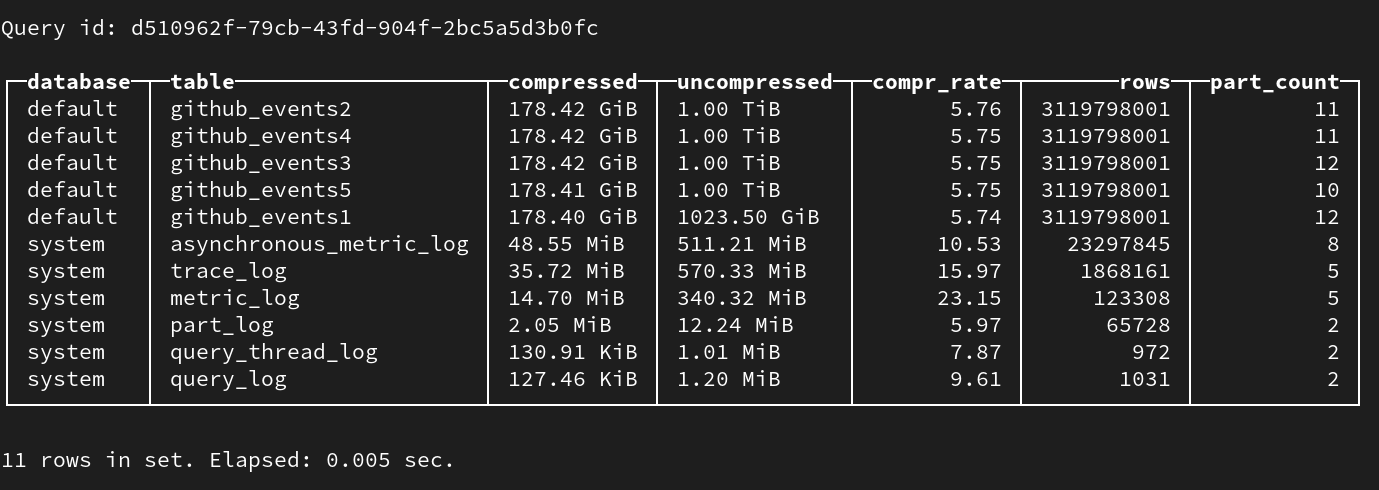
\includegraphics[width=.9\linewidth]{figures/clickhouse/table_size_local_backup.png}
\end{center}
\subsubsection{New attempt at downloading}
\label{sec:orgee99b19}
Delete local backup:
\begin{minted}[breaklines=true,breakanywhere=true]{bash}
./clickhouse-backup delete local 2022-05-11T07-25-16
# 2022/05/14 11:14:26.277665  info SELECT value FROM `system`.`build_options` where name='VERSION_INTEGER'
# 2022/05/14 11:14:26.280677  info SELECT * FROM system.disks;
# 2022/05/14 11:14:26.327285  info done                      backup=2022-05-11T07-25-16 duration=52ms location=local operation=delete
\end{minted}

List remote backups
\begin{minted}[breaklines=true,breakanywhere=true]{bash}
./clickhouse-backup list remote --config config.yaml
# 2022/05/14 11:15:16.688656  info SELECT max(toInt64(bytes_on_disk * 1.02)) AS max_file_size FROM system.parts
# 2022-05-11T07-25-16   895.29GiB   11/05/2022 10:44:05   remote      tar
# 2022-05-14T10-12-59   2.81KiB     14/05/2022 10:13:31   remote      tar
\end{minted}

Downloading the remote backup failed once again:
\begin{minted}[breaklines=true,breakanywhere=true]{bash}
time ./clickhouse-backup download 2022-05-11T07-25-16 --config config.yaml
# 2022/05/14 11:16:23.426432  info SELECT value FROM `system`.`build_options` where name='VERSION_INTEGER'
# 2022/05/14 11:16:23.428319  info SELECT * FROM system.disks;
# 2022/05/14 11:16:23.433846  info SELECT max(toInt64(bytes_on_disk * 1.02)) AS max_file_size FROM system.parts
# 2022/05/14 11:16:23.506743  info done                      backup=2022-05-11T07-25-16 duration=16ms operation=download size=3.36KiB table_metadata=default.github_events1
# 2022/05/14 11:16:23.512251  info done                      backup=2022-05-11T07-25-16 duration=5ms operation=download size=3.32KiB table_metadata=default.github_events2
# 2022/05/14 11:16:23.517891  info done                      backup=2022-05-11T07-25-16 duration=6ms operation=download size=3.36KiB table_metadata=default.github_events3
# 2022/05/14 11:16:23.522455  info done                      backup=2022-05-11T07-25-16 duration=5ms operation=download size=3.32KiB table_metadata=default.github_events4
# 2022/05/14 11:16:23.527403  info done                      backup=2022-05-11T07-25-16 duration=5ms operation=download size=3.28KiB table_metadata=default.github_events5
# 2022/05/14 11:17:23.532041 error can't acquire semaphore during downloadTableData: context canceled---------]  70.38% 59s
# 2022/05/14 11:17:23.697884 error can't acquire semaphore during Download: context canceled backup=2022-05-11T07-25-16 operation=download
# 2022/05/14 11:18:23.730339 error can't acquire semaphore during downloadTableData: context canceled---------]   9.31% 59s
# 2022/05/14 11:18:23.914406 error one of Download go-routine return error: one of downloadTableData go-routine return error: handling file: /all_3441_4218_4/push_distinct_size.bin: context deadline exceeded
#
# real    2m0.504s
# user    0m11.834s
# sys     0m16.363s
\end{minted}
